\section{if-else}
\label{sec:if}
\begin{frame}<beamer>
    \frametitle{Outline}
    \tableofcontents[currentsection]
\end{frame}


\begin{frame}\frametitle{if-else clause (1)}
\begin{itemize}
	\item {Read a character from input}
	\begin{enumerate}
		\item {If it is in 0$\sim$9, print out ``It is a digit''}
		\item {If it is in `a'$\sim$`z', convert it into upper case and print it out}
		\item {If it is in `A'$\sim$`Z', print it out directly}
		\item {If it is blank, print ``It is blank''}
		\item {Otherwise, print ``It is not a visible character''}
	\end{enumerate}
\end{itemize}
\end{frame}

\ifx\answer\undefined
\begin{frame}[fragile]\frametitle{if-else clause (2)}
\begin{lstlisting}[basicstyle=\large]
#include <stdio.h>
int main()
{
    char ch = ' ';
    ch = getchar();
    if(ch == ' ')
    {
        printf("It is blank\n");
    }else if(ch >= '0' && ch <= '9')
    {
        printf("It is digit\n");
    }
\end{lstlisting}
\end{frame}

\begin{frame}[fragile]\frametitle{if-else clause (3)}
\begin{lstlisting}[basicstyle=\large,firstnumber=13]
    else if(ch >= 'a' && ch <= 'z')
    {
        printf("%c", ch-32);
    }    
    else if(ch >= 'A' && ch <= 'Z')
    {
        printf("%c", ch);
    }else{
        printf("It is not visible character");
    }
    return 0;
}
\end{lstlisting}
\end{frame}
\fi

%\begin{frame}
%\frametitle{if-else clause (1)}
%\vspace{-0.15in}
%\begin{itemize}
%	\item {Convert a score (0$\sim$100) to A - E levels}
%	\begin{enumerate}
%		\item {90 - 100: A}
%		\item {80 - 89: B}
%		\item {70 - 79: C}
%		\item {60 - 69: D}
%		\item {  $<$ 60: E}
%	\end{enumerate}
%	\item {The input should be a float}
%	\item {Print out the resulting level to the screen}
%\end{itemize}
%\begin{center}
%	81 -----$>$ B
%\end{center}
%
%\end{frame}
%
%\begin{frame}
%\frametitle{if-else clause (2)}
%\vspace{-0.15in}
%	\begin{enumerate}
%		\item {\#include $<$stdio.h$>$}
%		\item {int~main(~)}
%		\item {\{}
%		\item {~~~float score = 0;}
%   		\item {~~~char grade = '0';}
%		\item {~~~printf("Please input scores: ");}
%		\item {~~~scanf("\%f", \&score);}
%		\item {~~~if(score $<$ 0 $\parallel$ score $>$ 100)}
%		\item {~~~\{}
%   		\item {~~~~~printf("Input is invalid!${\setminus}$n");}
%		\item {~~~\}}
%		\item {~~~else\{}
%		\item {~~~~~if(score $>=$ 90)}
%		\item {~~~~~~~~grade = 'A';}
%		\item {~~~~~else if(score $>=$ 80)\{}
%		\item {~~~~~~~~grade = 'B';}
%		\item {~~~~~~\}else if(score $>=$ 70)\{}
%	\end{enumerate}
%\end{frame}
%
%\begin{frame}
%\frametitle{if-else clause (2)-continued}
%\begin{enumerate}
%	\setcounter{enumi}{17}
%		\item {~~~~~~~~~grade = 'C';}
%		\item {~~~~~~\}else if(score $>=$ 60)\{}
%		\item {~~~~~~~~~grade = 'D';}
%		\item {~~~~~~\}else \{}
%		\item {~~~~~~~~~~grade = 'E';}
%		\item {~~~~~~~\}}
%		\item {~~~\}//if-else}
%		\item {~~~printf("\%5.1f ---$>$ \%c${\setminus}$n", score, grade);}
%		\item {\}}
%\end{enumerate}
%\end{frame}

\section{Embedded if-else}
\label{sec:if1}
\begin{frame}<beamer>
    \frametitle{Outline}
    \tableofcontents[currentsection]
\end{frame}

\begin{frame}
\frametitle{Embedded if-else}
\vspace{-0.1in}
\begin{itemize}
	\item {Given the height and gender of a student, recommend a sport for him/her}
\end{itemize}
\begin{figure}
	\begin{center}
		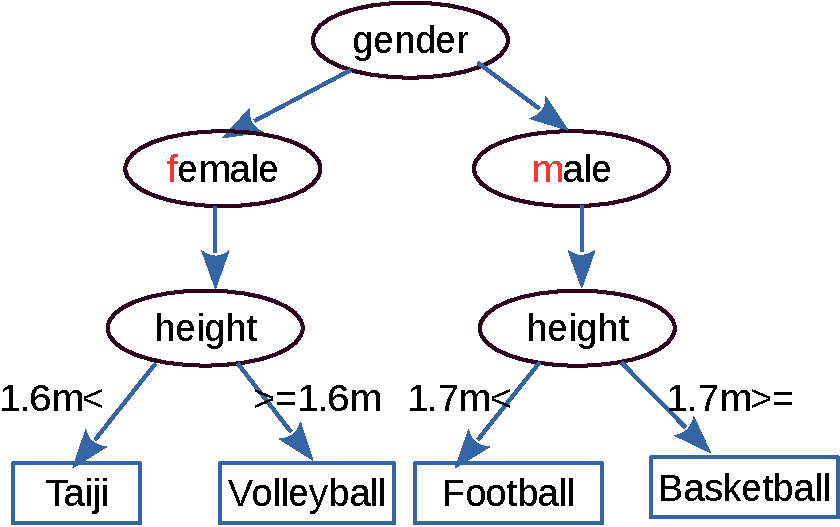
\includegraphics[width=0.45\linewidth]{figs/sports.pdf}
	\end{center}
\end{figure}
\begin{itemize}
	\item {For exapmle, given male student with height 1.75m, it is recommended to play basketball}
	\item {Th input is \textcolor{red}{m}/\textcolor{red}{f} for gender, and a positive float number for height}
	\item {The output is the recommended sports name}
\end{itemize}
\end{frame}

\ifx\answer\undefined
\begin{frame}[fragile]{The answer (1)}
\begin{lstlisting}[xleftmargin=0.05\linewidth]
#include <stdio.h>
int main( )
{
  char gender = ' ';
  float height = 0.0;
  printf("Please input gender: ");
  scanf("%c", &gender);
  printf("Please input height: ");
  scanf("%f", &height);
  if(gender == 'm')
  {
     if(height >= 1.70)
     {
         printf("Basketball\n");
     }else
\end{lstlisting}
\end{frame}
\fi

\ifx\answer\undefined
\begin{frame}[fragile]{The answer (2)}
\begin{lstlisting}[xleftmargin=0.05\linewidth, firstnumber=16]
     {
         printf("Football\n");
     }
  }else if(gender == 'f')
  {
     if(height >= 1.60)
     {
         printf("Volleyball\n");
     }else
     {
         printf("Taiji\n");
     }
  }//else-if(gender)
}

\end{lstlisting}
\end{frame}
\fi

\section{switch-case}
\label{sec:if}
\begin{frame}<beamer>
    \frametitle{Outline}
    \tableofcontents[currentsection]
\end{frame}

\begin{frame}
\frametitle{switch clause}
\begin{itemize}
	\item {Write C codes, which allows user to input number between 1 and 12 (the month)}
	\item {Then your code tells the user to which season the input month belongs}
\end{itemize}
\begin{center}
\begin{enumerate}
	\item {2---4 : Spring}
	\item {5---7 : Summer}
	\item {8---10 : Autumn}
	\item {12---1 : Winter}
\end{enumerate}
\end{center}
\end{frame}

\ifx\answer\undefined
\begin{frame}[fragile]
\begin{lstlisting}[xleftmargin=0.05\linewidth]
#include <stdio.h>
int main( )
{
  int m = 0;
  printf("Please input month: ");
  scanf("%d", &m);
  if(m < 1 || m > 12)
  {
    printf("The input is invalid!\n");}
  } else
  {
   switch(m)
   {
     case 2:
     case 3:
     case 4: printf("%d --- Spring\n", m); break;
\end{lstlisting}
\end{frame}
\fi

\ifx\answer\undefined
\begin{frame}[fragile]
	\begin{lstlisting}[xleftmargin=0.05\linewidth, firstnumber=15]
     case 5:
     case 6:
     case 7:printf("%d --- Summer\n", m); break;
     case 8:
     case 9:
     case 10:printf("%d --- Autumn\n", m); break;
     case 11:
     case 12:
     case 1: printf("%d --- Winter\n", m); break;
   }//end-switch
  }//end-else
}//end-main
	\end{lstlisting}
\end{frame}
\fi
